%! Author = josephbeal
%! Date = 3/25/25

% Preamble
\documentclass[11pt]{texMemo}

% Packages
\usepackage{amsmath,hyperref}
\usepackage{booktabs}
\usepackage{graphicx}
\usepackage{dcolumn} % Required for D column specifier

\memosubject{Data Exercise 2 Memo}
\memofrom{Patrick Beal}
\memodate{\today}

% Document
\begin{document}
\maketitle

\section{Introduction}
We seek to explore the impact of various technological developments on the growth in per capita GDP between developed and developing countries.
In particular, we examine the impact of cellphones, tractor usage, hospital beds, cars, and transactions using payment cards.
Technology has developed at exponential rates over the past few decades and does not appear to be slowing down.
With it, we have seen drastic increases in the disparity in wealth and living conditions, especially between developed and developing countries.
Because GDP growth can be a proxy for the standard of living, exploring the relationship between technology and GDP growth can help identify where efforts will be most effective in improving the standard of living in developing nations.

We use international GDP data and technology data to estimate these effects, and we will use a regression analysis to quantify the impacts.
We selected France, Germany, Italy, Japan, the United Kingdom, and the United States as developed countries, and left everything else as developing countries.

\section{Data}
\subsection{Data Sources}
We used two primary datasets in our analysis.
First, we used the Penn World Table version 10.01, developed by the Groningen Growth and Development Centre at the University of Groningen's Faculty of Economics and Business.
The data can be found at \href{https://www.rug.nl/ggdc/productivity/pwt/}{here}.
This dataset provides a comprehensive set of data on GDP and other economic indicators for over 200 countries, including both developed and developing nations.
We used the data on GDP per capita in constant 2017 US dollars, which allows us to compare the economic performance of different countries over time.

Second, we used the Cross-country Historical Adoption of Technology (CHAT) dataset, from the National Bureau of Economic Research (NBER), found at this \href{https://data.nber.org/data-appendix/w15319/}{link}.
This dataset provides information on the adoption of various technologies across countries and over time, from which we choose to include cellphones, tractors, hospital beds, cars, and payment card transactions.
We choose these variables because they are representative of technological advancements across multiple domains: communications, agriculture, healthcare, transportation, and finance.

\subsection{Data Cleaning}
Our first step was to merge the two datasets and create binary variables indicating whether a country was developed or not, using the countries listed above.
We used the country codes provided in both datasets to match the data on GDP with the data on technology adoption.
We then calculated the GPD per capita by dividing the GDP by the population for each country and year.
To compare developed and developing countries, we took the population-weighted average of all of our variables of interest for each country and year.

To calculate the growth rate of GDP per capita, we took the difference of the logarithm of each of our variables of interest.
Specifically, we calculated
\begin{align*}
    \text{GDP per capita Growth Rate} &= \Delta \log(\text{GDP}/\text{pop}) \\
    &= \log(\text{GDP}/\text{pop})_t - \log(\text{GDP}/\text{pop})_{t-1}.
\end{align*}

We also created interaction terms between the binary variable for developed countries and each of the technology variables. This allows us to estimate whether the impact of technology on GDP growth differs between developed and developing countries. 
Finally, we retained only the variables needed for analysis, and filled missing values with zeros in the cell phone column.
This is justified because the missing values indicated years before cell phones had been created, so it's safe to assume that nobody in those years had cell phones.

Altogether we ended up with the following variables.
\begin{itemize}
    \item \textbf{GDP per capita growth rate}: The growth rate of GDP per capita, calculated as the difference in the logarithm of GDP per capita between two consecutive years.
    \item \textbf{Cellphones}: The number of users of portable cell phones.
    \item \textbf{Tractors}: The number of wheel and crawler tractors used in agriculture.
    \item \textbf{Hospital beds}: The number of hospital beds, including inpatient beds available in public, private, general, and specialized hospitals and rehabilitation centers.
    \item \textbf{Cars}: The number of passenger cars (excluding tractors and commercial vehicles). These numbers are reported from registration and licensing records.
    \item \textbf{Electronic Funds Transfer}: The number of transactions using payment cards, including debit and credit cards.
    \item \textbf{Average Annual Hours Worked}: The average number of hours worked per person in a given year and country.
    \item \textbf{Human Capital Index}: Human capital index as calculated by years of schooling and returns to education.
    \item \textbf{Population}: The average population of the category (developed or developing) in a given year.
    \item \textbf{Percentage of Literacy}: The percentage of the population that is literate.
    \item \textbf{Developed}: A binary variable indicating whether a country is developed (1) or developing (0).
    \item \textbf{Developed Country Interactions}: Interaction terms between the developed binary variable and each of the technology variables. This allows us to estimate whether the impact of technology on GDP growth differs between developed and developing countries.
    \item \textbf{Logarithms and Growth Rates}: For each of these values, we had the original values, the logarithm of the values, and the growth rate of the values, calculated using similar formulas to that given for the GDP growth rate.
    \item \textbf{Year}: The year of the observation.
\end{itemize}
We treated GDP per capita growth rate as our dependent variable, and the rest of the variables as independent variables.
Cellphones, tractors, hospital beds, cars, and electronic funds transfer were our primary independent variables of interest, while average annual hours worked, human capital index, population, percentage of literacy, and the developed binary variable were our control variables.
We also included the interaction terms between the developed binary variable and each of the technology variables to estimate whether the impact of technology on GDP growth differs between developed and developing countries.

\subsection{Strengths and Limitations}
One weakness of our data is that we have a relatively small sample size—only about 54 samples, while many of the samples are zero because the technology in question had not yet been developed.
Moreover, the data is not perfectly accurate, as it is based on estimates and projections rather than perfect measurements.
Even those based on official government records, such as car data, cannot possibly know whether all the registered vehicles are actually in use, and there may be vehicles that are not registered.
However, the data is still useful for our analysis, as it provides a good overview of the trends in technology adoption and GDP growth over time.

We also have a few strengths in our data.
We have many variables to choose from, which allows us to control for many potential confounding variables.
Additionally, we have data on many countries, allowing us robust estimates of the average effect between developed and developing countries.


\subsection{Figures}
The plots in Figure~\ref{fig:all_plots} show the trends in the growth rates of GDP per capita and the technology adoption rates over time, for both developed and developing countries.

\begin{figure}[htbp]
    \centering
        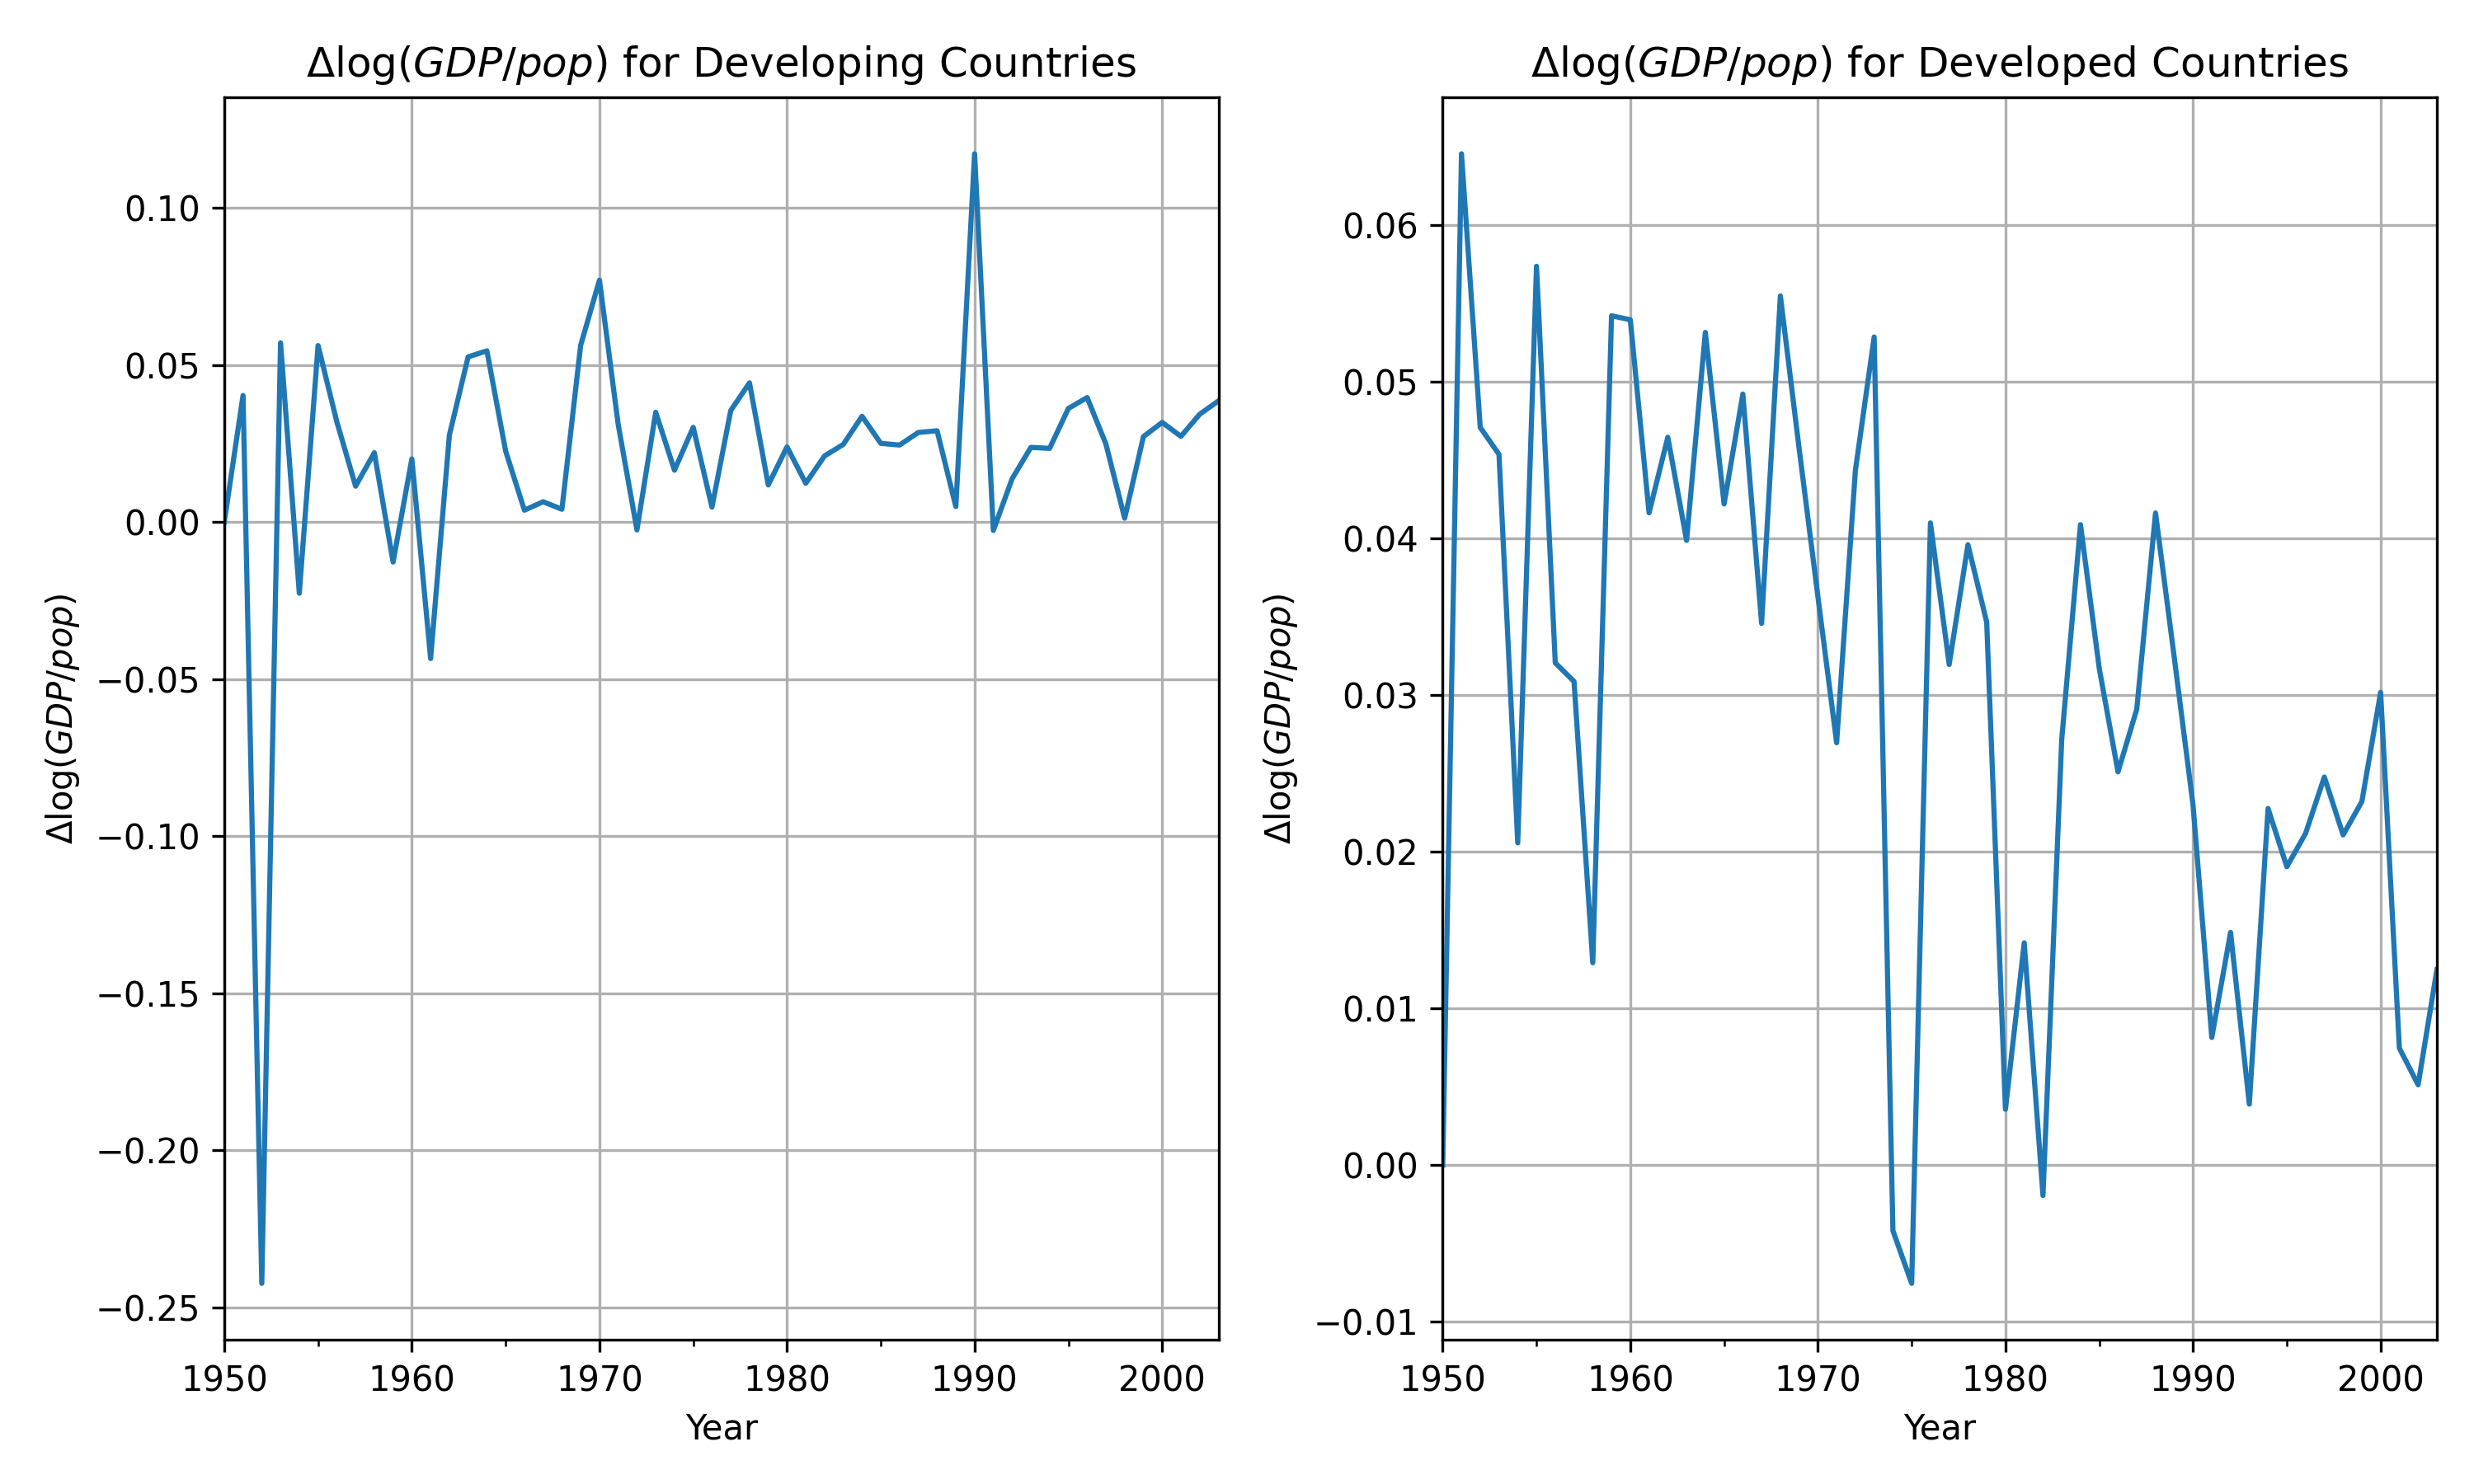
\includegraphics[width=0.45\textwidth]{figures/g_gdp_per_cap.png}
        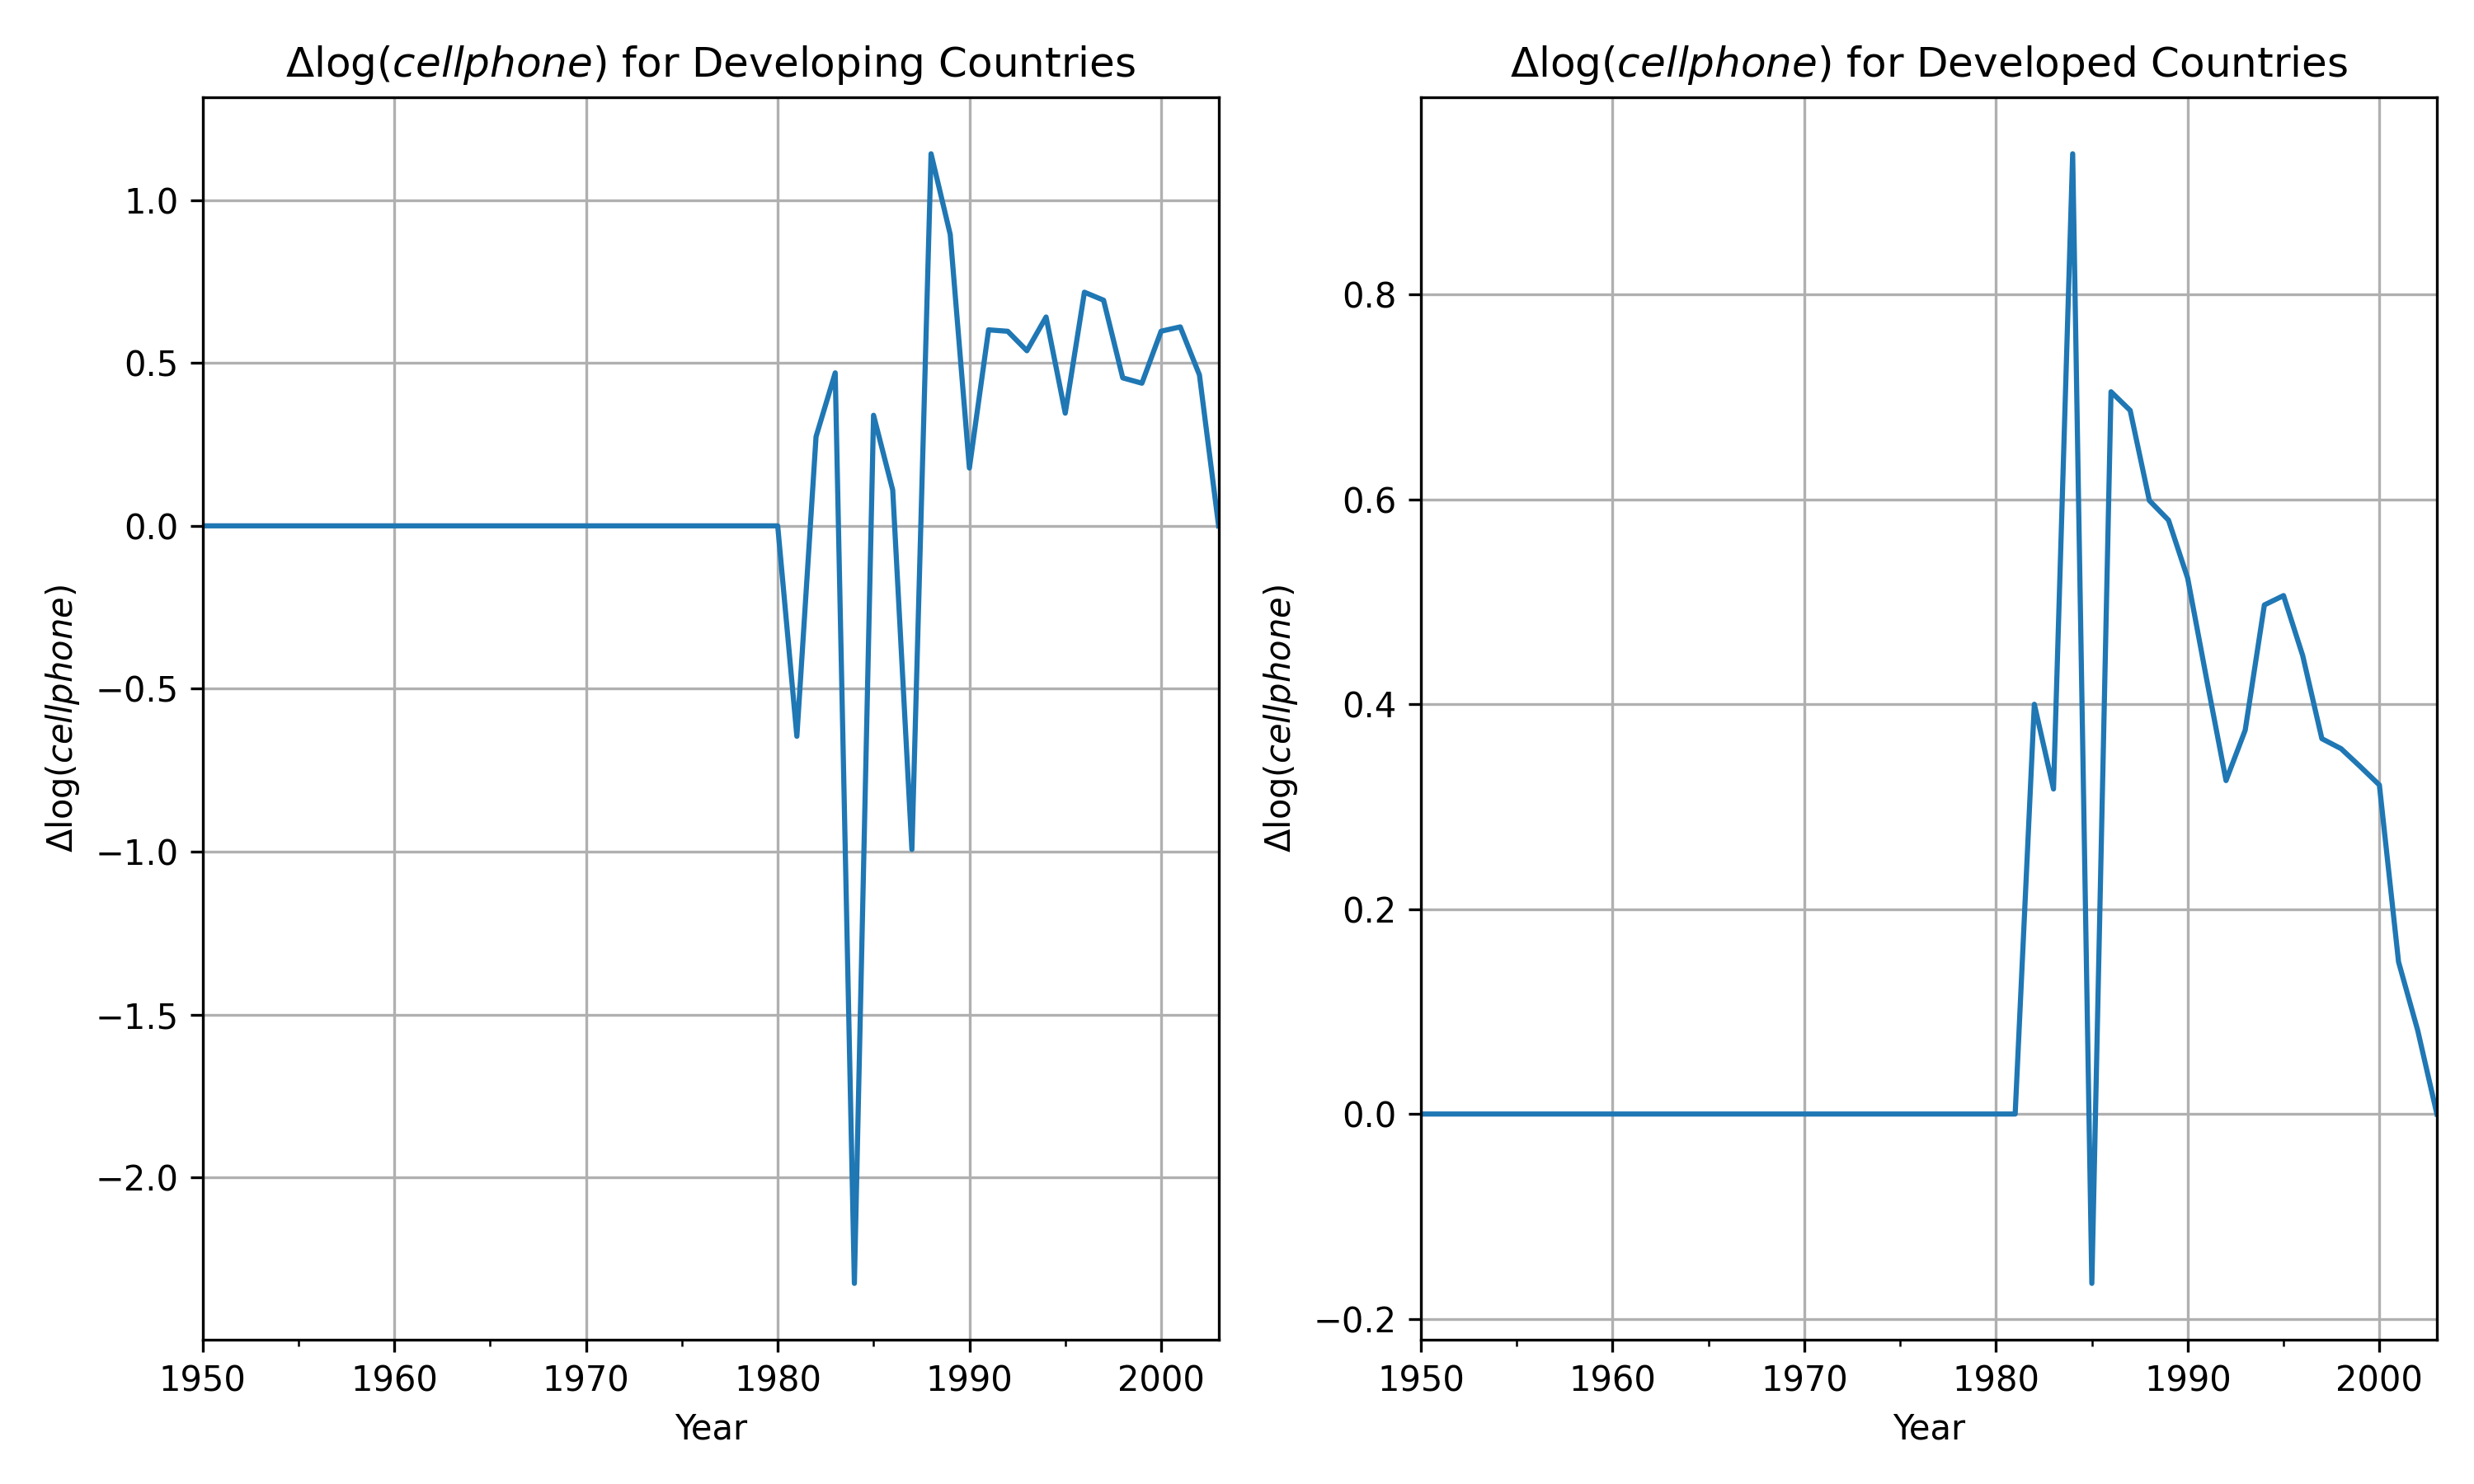
\includegraphics[width=0.45\textwidth]{figures/g_cellphone.png}
        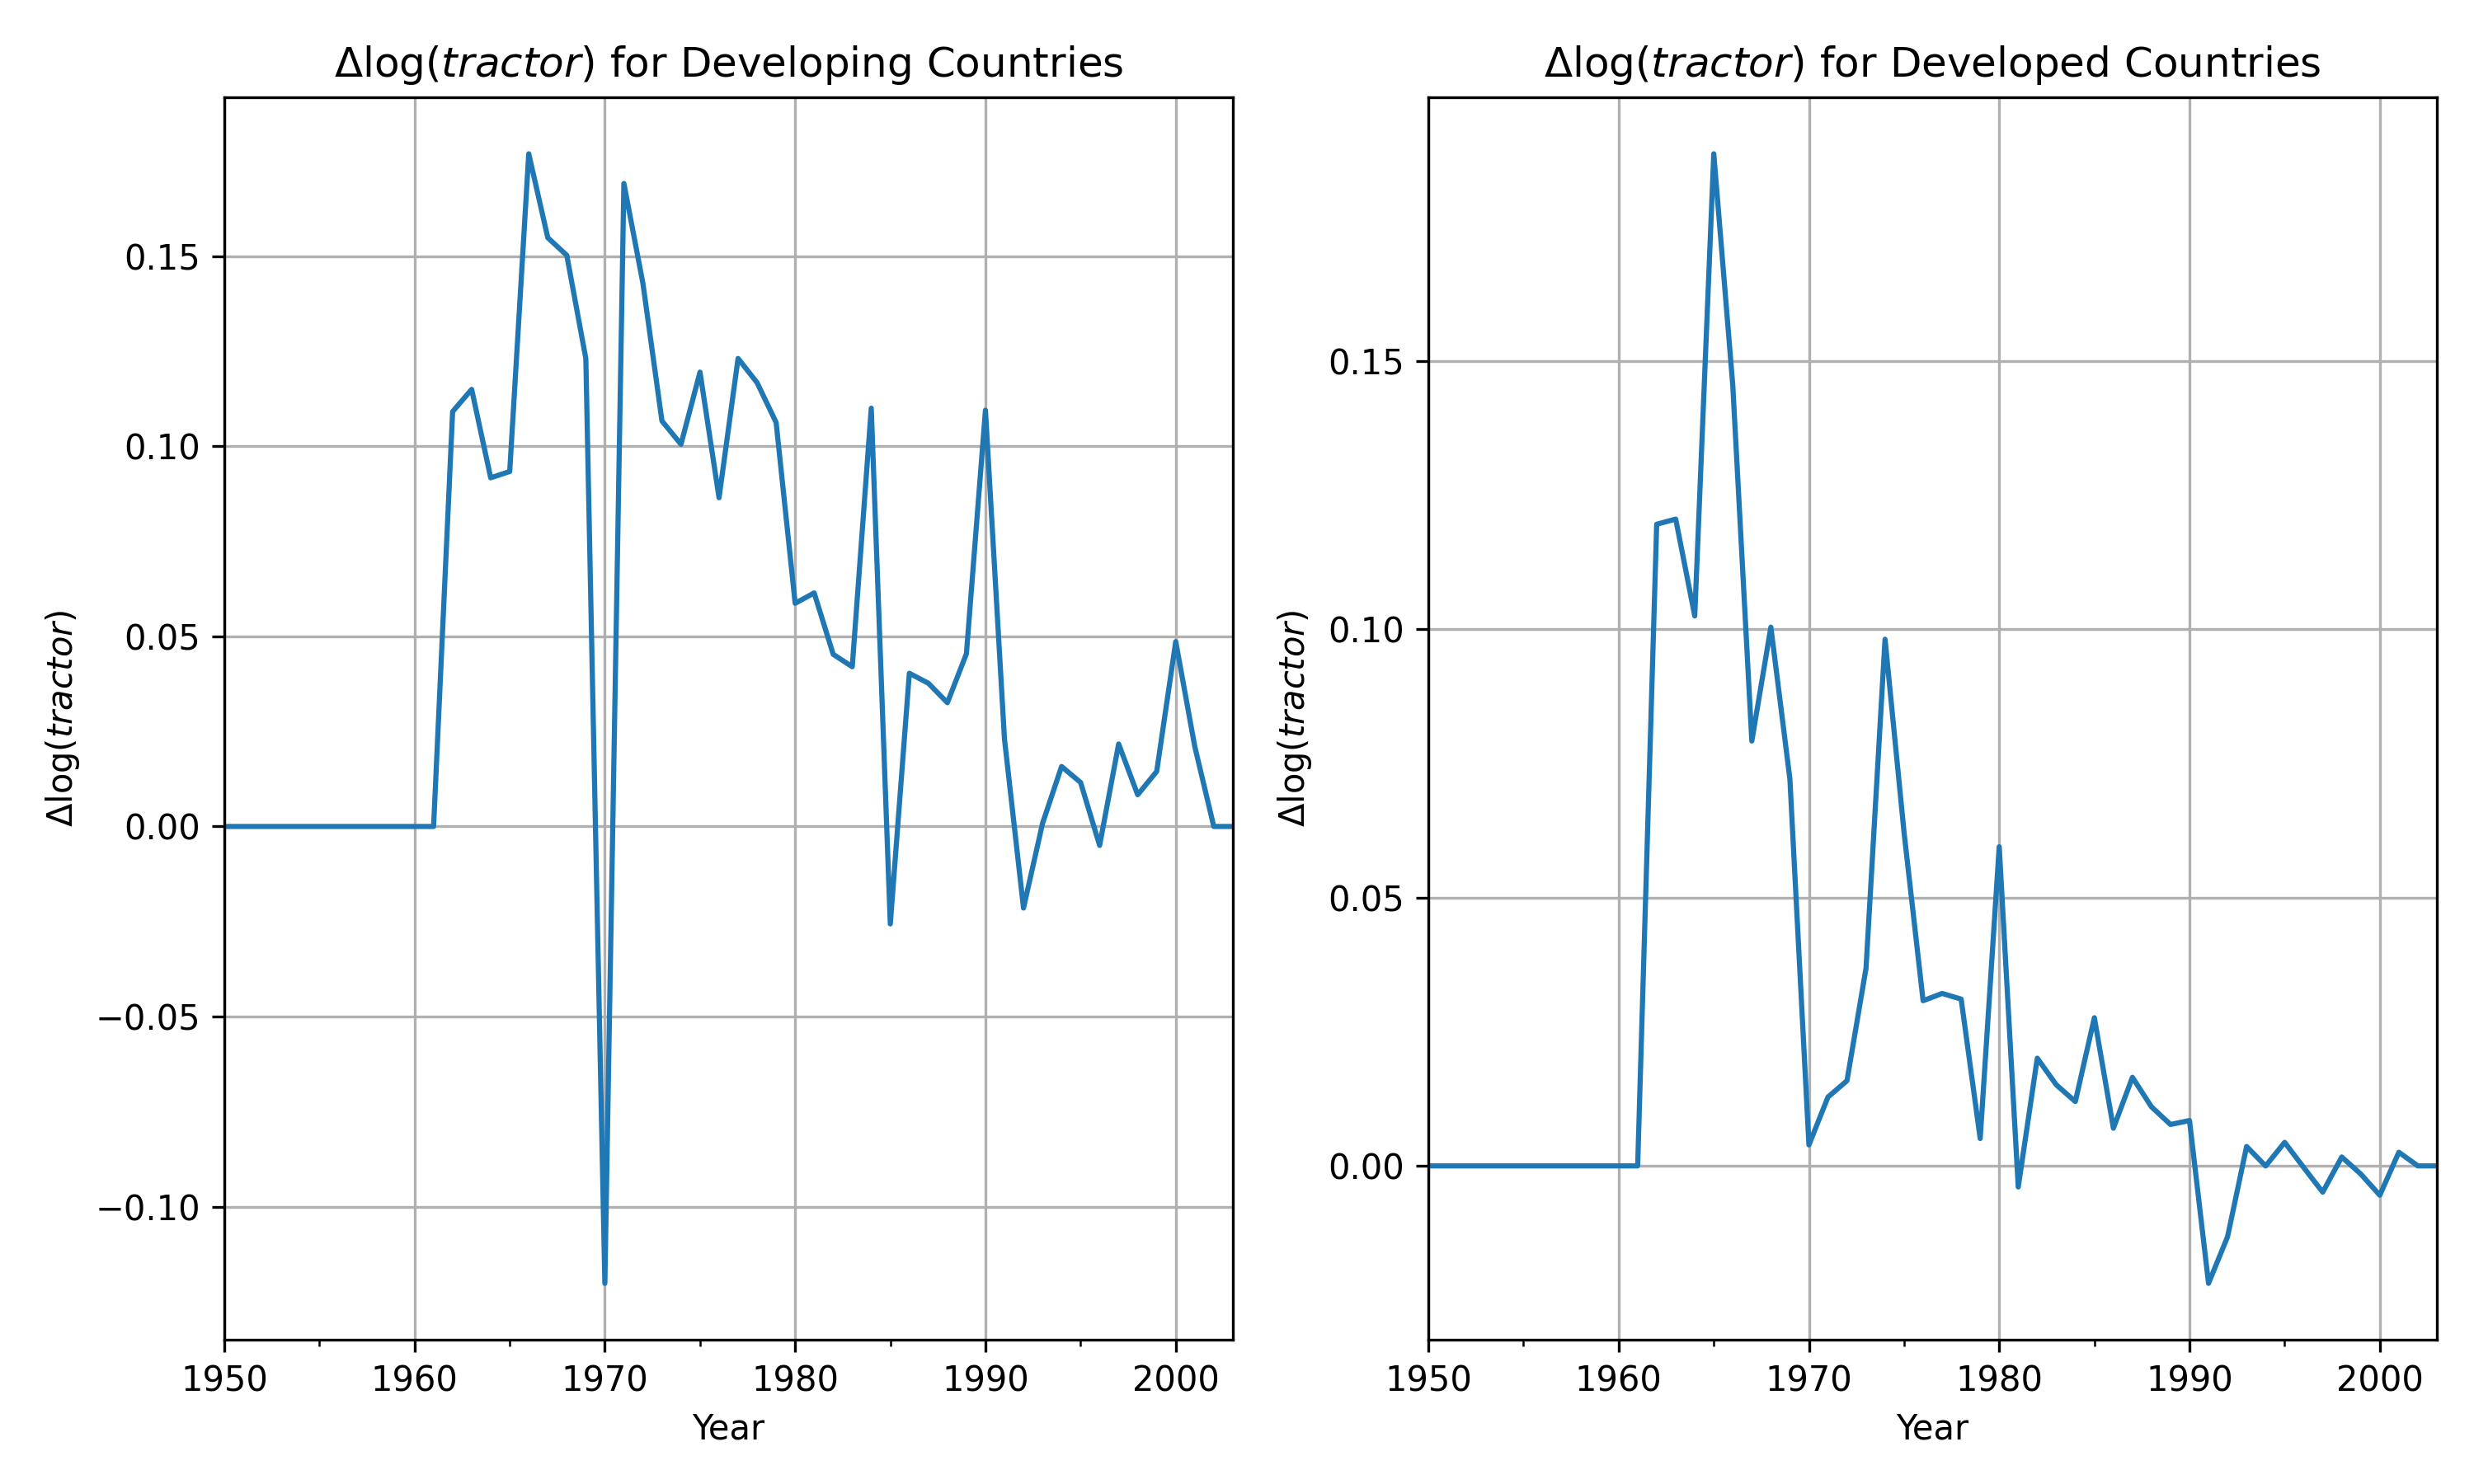
\includegraphics[width=0.45\textwidth]{figures/g_ag_tractor.png}
        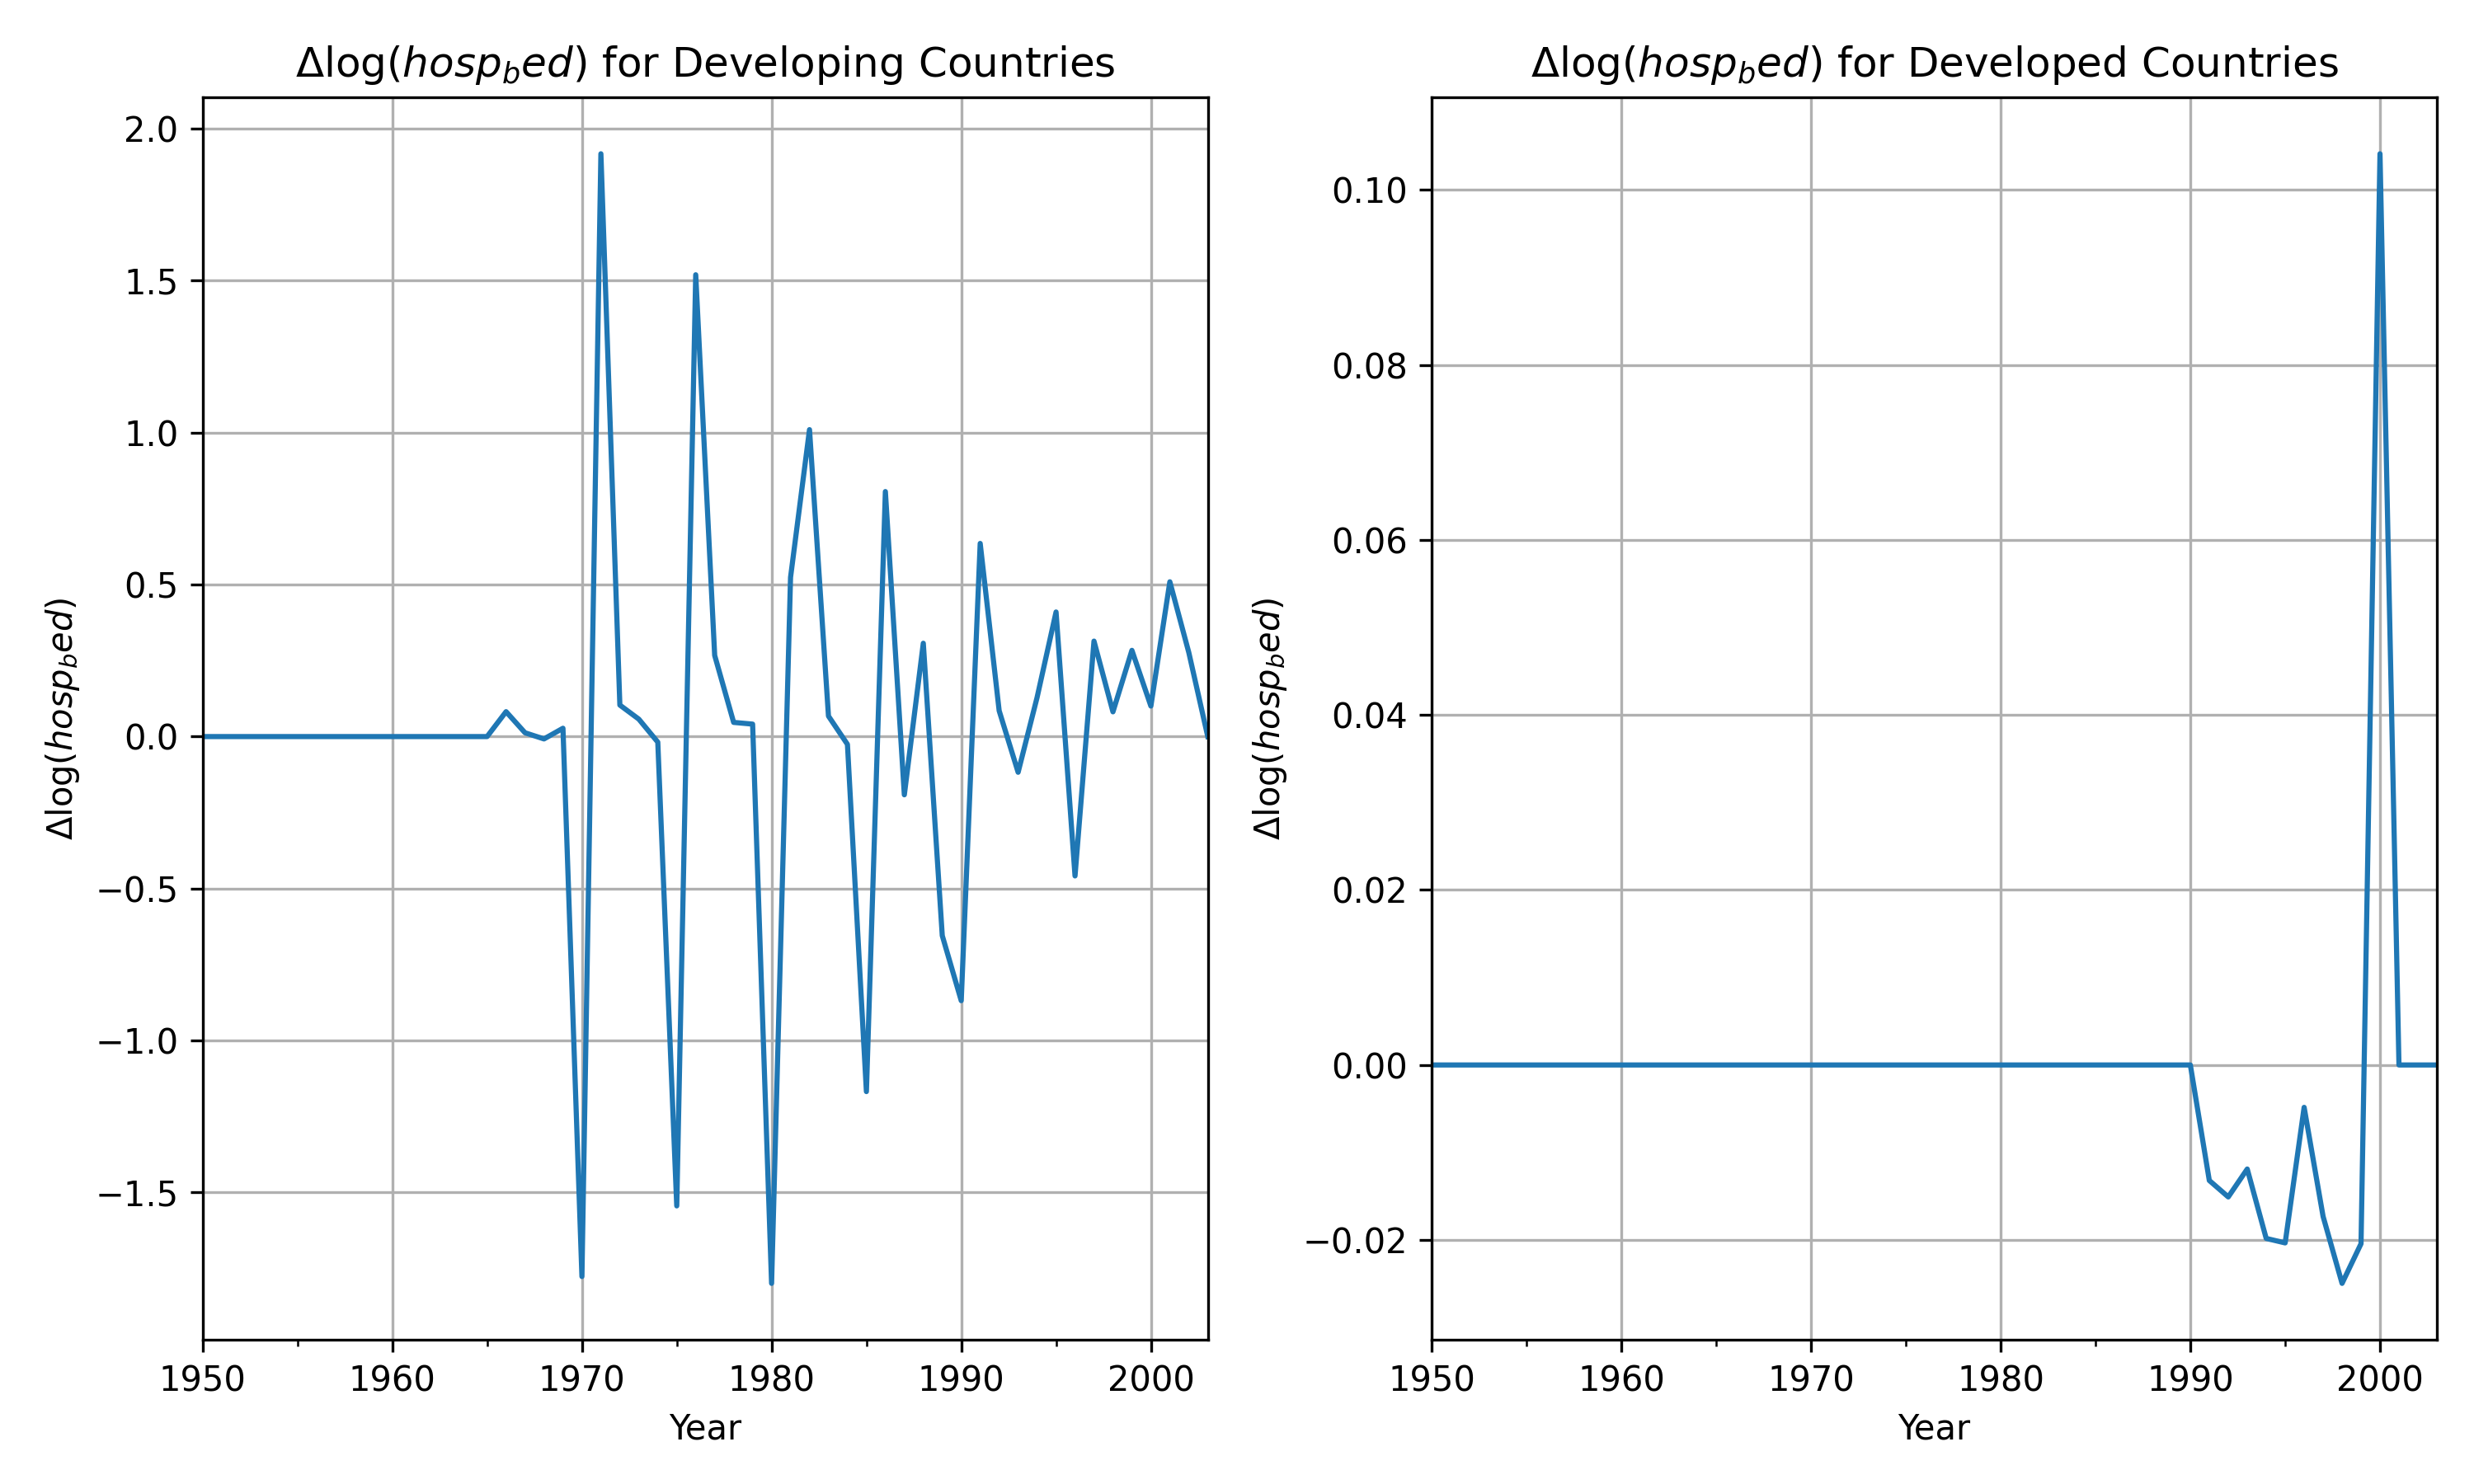
\includegraphics[width=0.45\textwidth]{figures/g_bed_hosp.png}
        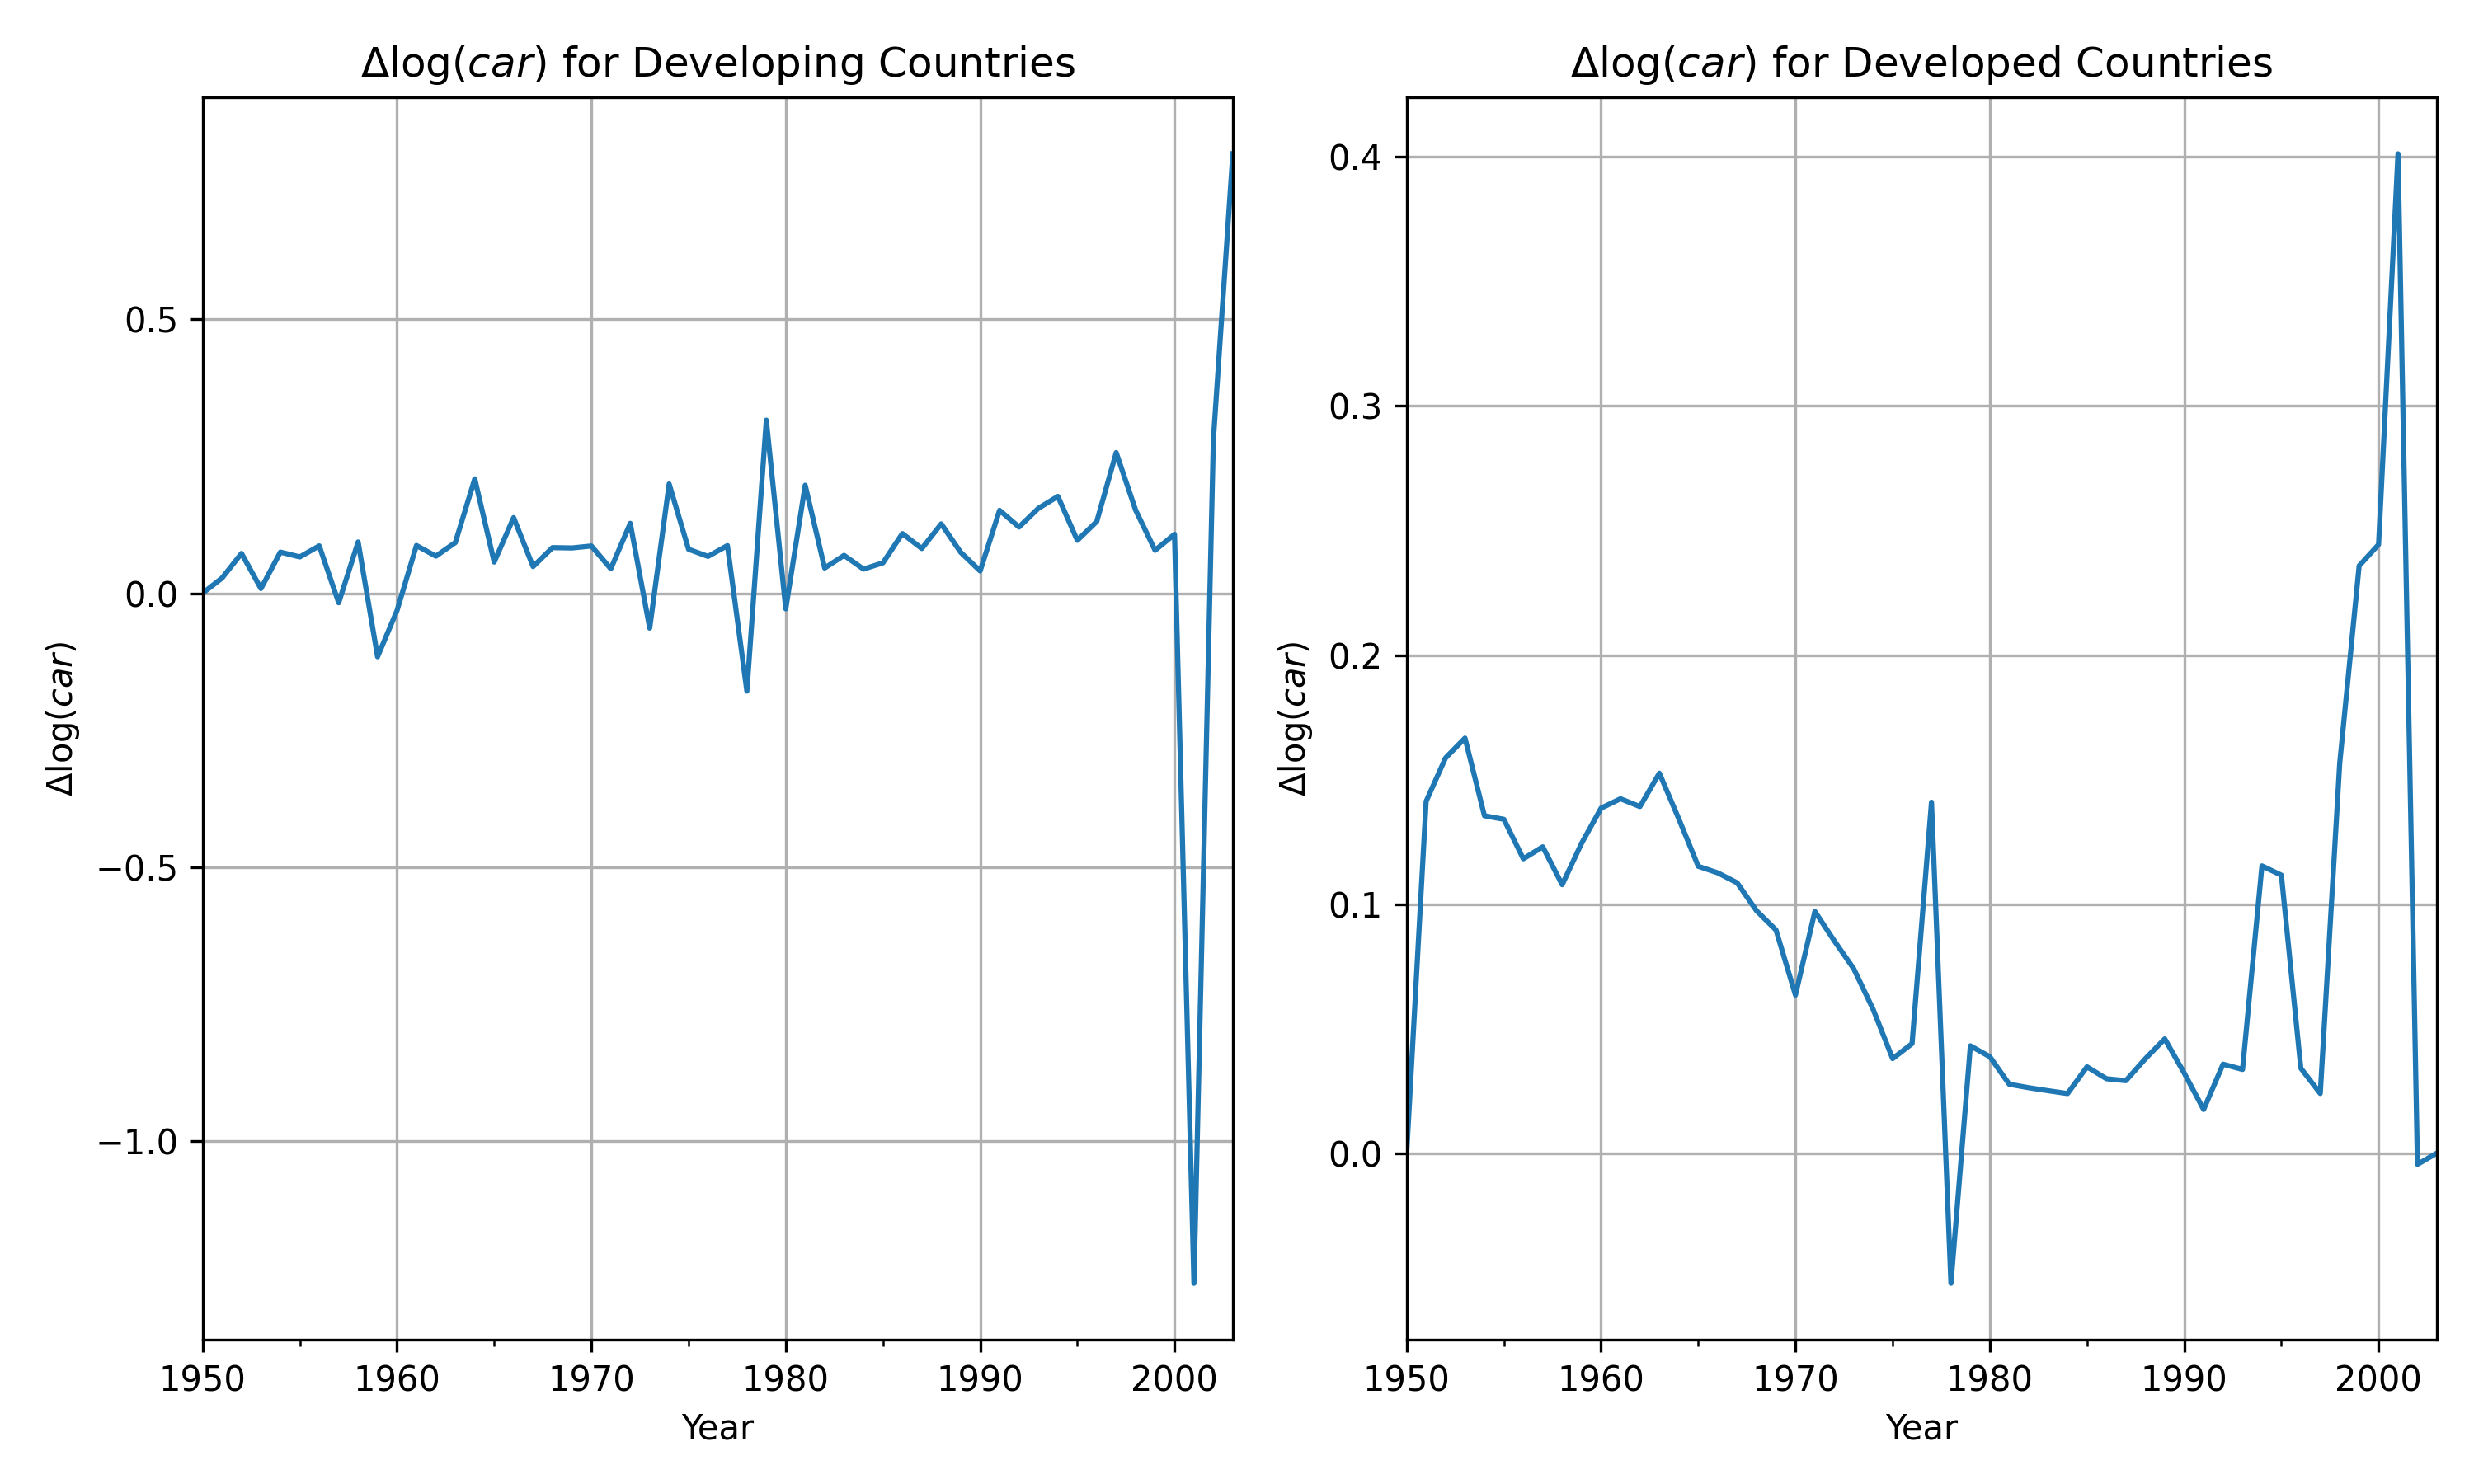
\includegraphics[width=0.45\textwidth]{figures/g_vehicle_car.png}
        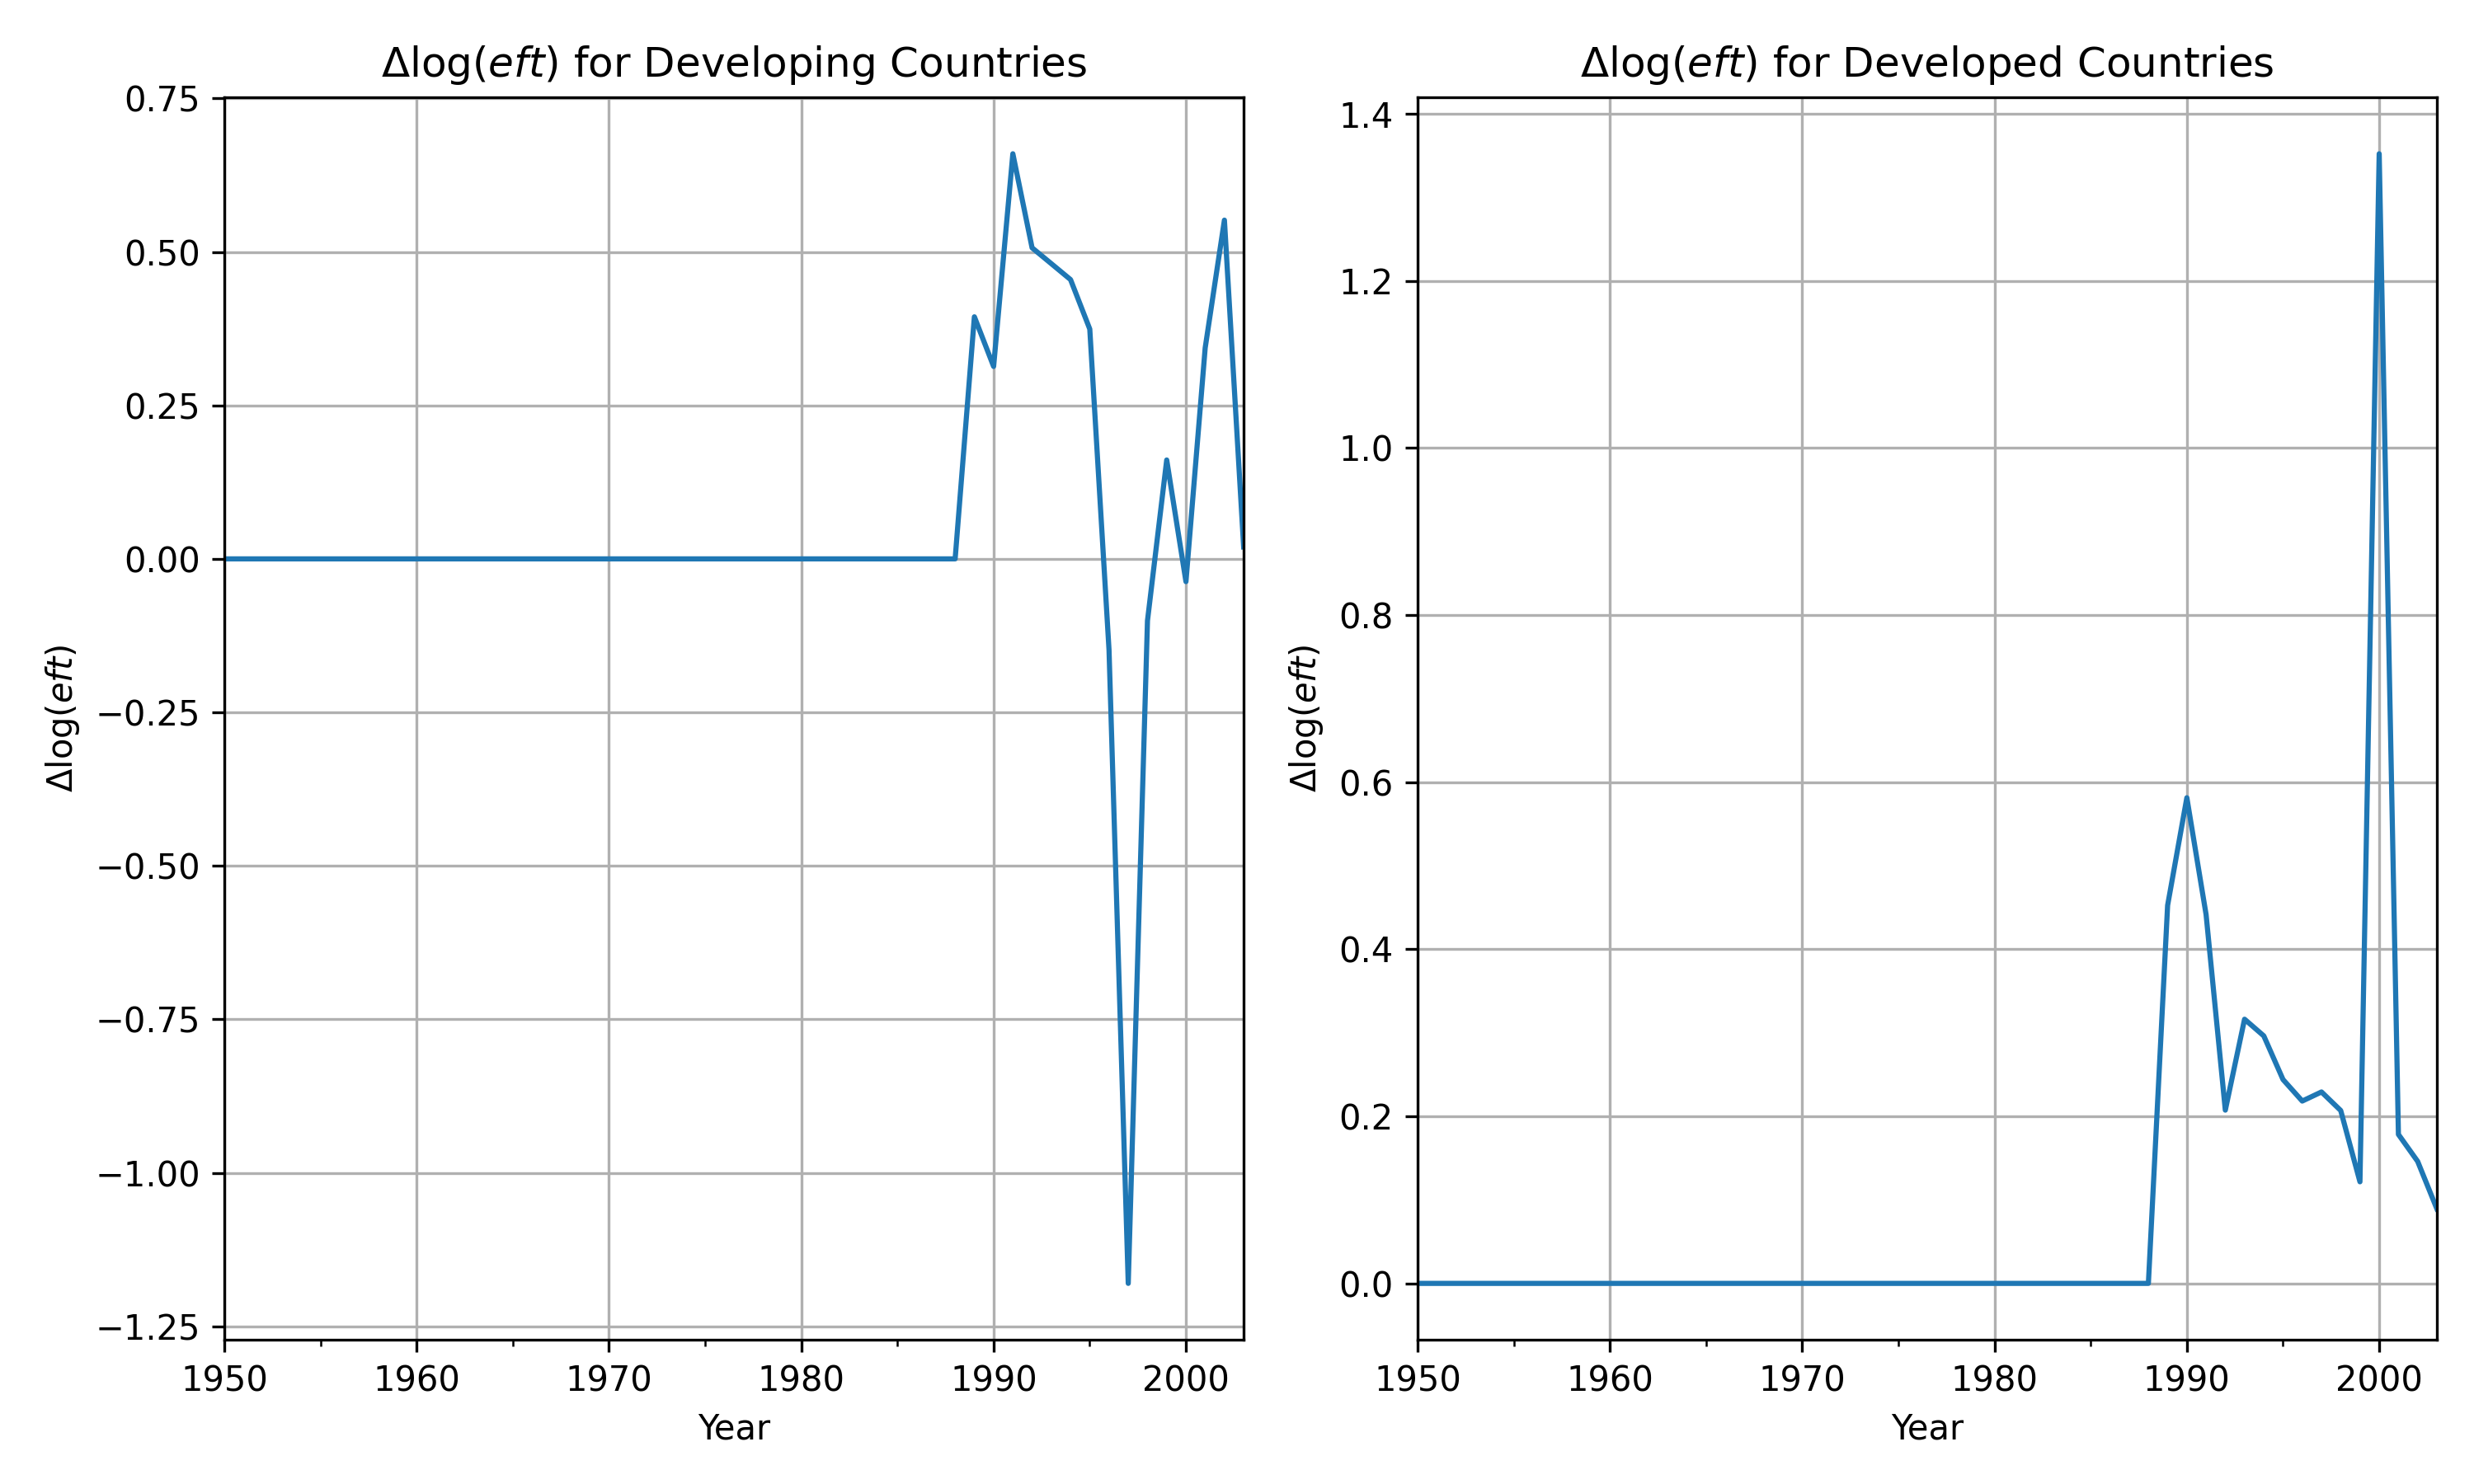
\includegraphics[width=0.45\textwidth]{figures/g_eft.png}
        \caption{Various plots illustrating the relationships between technology adoption and GDP growth.}
        \label{fig:all_plots}
        \end{figure}


\section{Empirical Analysis}

To make inferences about the causal impact of technology on GDP growth, we must be careful about our assumptions.
First, we assume that the relationship between technology and GDP growth is linear, which may not be the case.
We include interaction terms in a later regression to account for some potential differences in relationships.
Some of the results (such as including a squared time term) were shown to be insignificant both individually and jointly with other variables of interest, so we feel confident that those terms need not be included in the regression.
We also assume that the independent variables are exogenous and not correlated with the error term, which we cannot test.
Without this assumption, we cannot make causal inferences about the relationship between technology and GDP growth.
It is also important that we have no multicolinearity in the data, which our data satisfies.
This is because we included technology and other variables that are representative of different domains.
Had all our variables been related to phone communication, for example, we risk having multicolinearity.
We also assume that the error term is normally distributed and homoskedastic, though we avoid issues if this assumption fails by computing robust standard errors.

Most challenging is the exogeneity assumption.
We cannot assume that the technology variables are randomly assigned, so our best hope of satisfying this assumption is to control for as potentially confounding variables.

We ran multiple regressions to estimate the impact of technology on GDP growth, using a hierarchical model to control for the effects of other variables.
We first ran a regression with only the technology variables, and then added the control variables (not including the developed binary or the year) to see how they affected the results.
We then added the developed binary variable, followed by the year.
The results of this regression are shown in Table \ref{normal_reg}.

\begin{table}[htbp]\centering
\def\sym#1{\ifmmode^{#1}\else\(^{#1}\)\fi}
\caption{Effect of Technology Growth on GDP per Capita Growth}
\begin{tabular}{l*{4}{D{.}{.}{-1}}}
\hline\hline
                &\multicolumn{1}{c}{(1)}&\multicolumn{1}{c}{(2)}&\multicolumn{1}{c}{(3)}&\multicolumn{1}{c}{(4)}\\
                &\multicolumn{1}{c}{$\Delta \log(\text{GDP}/\text{pop})$}&\multicolumn{1}{c}{$\Delta \log(\text{GDP}/\text{pop})$}&\multicolumn{1}{c}{$\Delta \log(\text{GDP}/\text{pop})$}&\multicolumn{1}{c}{$\Delta \log(\text{GDP}/\text{pop})$}\\
\hline
$\Delta \log(\text{cellphone})$     &  0.00145         & -0.00454         & -0.00637\sym{*}  & -0.00281         \\
                &(0.00515)         &(0.00413)         &(0.00355)         &(0.00244)         \\
[1em]
$\Delta \log(\text{tractor})$    &   0.0782         & -0.00817         & -0.00113         &  -0.0137         \\
                & (0.0703)         & (0.0449)         & (0.0424)         & (0.0436)         \\
[1em]
$\Delta \log(\text{hosp\_bed})$      &  -0.0119\sym{*}  & -0.00635         & -0.00772\sym{*}  & -0.00718\sym{*}  \\
                &(0.00654)         &(0.00403)         &(0.00409)         &(0.00393)         \\
[1em]
$\Delta \log(\text{car})$   &  0.00635         &  0.00382         &-0.000206         & 0.000393         \\
                &(0.00989)         &(0.00692)         &(0.00868)         & (0.0111)         \\
[1em]
$\Delta \log(\text{eft})$           &  0.00152         & -0.00213         & -0.00331         &  0.00229         \\
                &(0.00742)         &(0.00686)         &(0.00583)         &(0.00534)         \\
[1em]
$\Delta \log(\text{avh})$           &                  &    0.403         &    0.848         &    0.875         \\
                &                  &  (0.387)         &  (0.592)         &  (0.562)         \\
[1em]
$\Delta \log(\text{hc})$            &                  &    1.841\sym{***}&    2.298\sym{***}&    2.580\sym{***}\\
                &                  &  (0.343)         &  (0.340)         &  (0.360)         \\
[1em]
$\Delta \log(\text{pop})$           &                  &   -0.154\sym{***}&   -0.115\sym{***}&  -0.0982\sym{***}\\
                &                  & (0.0280)         & (0.0302)         & (0.0315)         \\
[1em]
$\Delta \log(\text{pctivliteracy})$ &                  &  0.00371         &  0.00151         &  0.00105         \\
                &                  &(0.00688)         &(0.00583)         &(0.00551)         \\
[1em]
dev       &                  &                  &   0.0160\sym{***}&   0.0161\sym{***}\\
                &                  &                  &(0.00481)         &(0.00471)         \\
[1em]
Year            &                  &                  &                  &-0.000302\sym{**} \\
                &                  &                  &                  &(0.000126)         \\
[1em]
Constant        &   0.0213\sym{***}&   0.0144\sym{***}&  0.00364         &    0.597\sym{**} \\
                &(0.00613)         &(0.00411)         &(0.00543)         &  (0.252)         \\
\hline
Observations    &      108         &      108         &      108         &      108         \\
\hline\hline
\multicolumn{5}{l}{\footnotesize Standard errors in parentheses}\\
\multicolumn{5}{l}{\footnotesize \sym{*} \(p<0.10\), \sym{**} \(p<0.05\), \sym{***} \(p<0.01\)}\\
\end{tabular}
\label{normal_reg}
\end{table}


From these regressions, we see that the technology variables are significantly insignificant.
The change in human capital rate and the change in the population growth rate are highly significant ($p < 0.01$) in all models they are included in, as is the binary variable for developed countries.
This indicates that there is not significant evidence that technological growth leads to GDP growth.

We also ran regressions including the interaction terms between the developed binary variable and each of the technology variables to estimate whether the impact of technology on GDP growth differs between developed and developing countries.
The results of this regression are shown in Table \ref{by_developed}.

\begin{table}[htbp]\centering
\def\sym#1{\ifmmode^{#1}\else\(^{#1}\)\fi}
\caption{Effect of Technology Growth on GDP per Capita Growth by Developed}
\begin{tabular}{l*{3}{D{.}{.}{-1}}}
\hline\hline
                &\multicolumn{1}{c}{Developing}&\multicolumn{1}{c}{Developed}&\multicolumn{1}{c}{Both}\\
                &\multicolumn{1}{c}{$\Delta \log(\text{GDP}/\text{pop})$}&\multicolumn{1}{c}{$\Delta \log(\text{GDP}/\text{pop})$}&\multicolumn{1}{c}{$\Delta \log(\text{GDP}/\text{pop})$}\\
\hline
$\Delta \log(\text{cellphone})$     & -0.00259         & -0.00115         & -0.00368         \\
                &(0.00295)         &(0.00603)         &(0.00288)         \\
[1em]
$\Delta \log(\text{tractor})$    &   0.0205         &  -0.0314         &  -0.0161         \\
                & (0.0674)         & (0.0337)         & (0.0628)         \\
[1em]
$\Delta \log(\text{hosp\_bed})$      & -0.00475         &    0.229\sym{**} & -0.00711\sym{*}  \\
                &(0.00350)         & (0.0927)         &(0.00400)         \\
[1em]
$\Delta \log(\text{car})$   & -0.00397         &   0.0148         & -0.00455         \\
                &(0.00898)         & (0.0111)         & (0.0107)         \\
[1em]
$\Delta \log(\text{eft})$           & -0.00324         &  -0.0118         &-0.000426         \\
                &(0.00748)         &(0.00966)         &(0.00771)         \\
[1em]
$\Delta \log(\text{avh})$           &   -0.249         &    2.107\sym{***}&    0.825         \\
                &  (0.492)         &  (0.355)         &  (0.556)         \\
[1em]
$\Delta \log(\text{hc})$            &    1.959\sym{***}&    3.433\sym{***}&    2.556\sym{***}\\
                &  (0.538)         &  (0.928)         &  (0.409)         \\
[1em]
$\Delta \log(\text{pop})$           &   -0.141\sym{***}&    1.783\sym{***}&  -0.0995\sym{***}\\
                & (0.0366)         &  (0.591)         & (0.0334)         \\
[1em]
$\Delta \log(\text{pctivliteracy})$ &  0.00718         &   -1.006\sym{***}&  0.00144         \\
                &(0.00648)         &  (0.314)         &(0.00565)         \\
[1em]
Year            &0.00000216         &-0.000114         &-0.000260         \\
                &(0.000297)         &(0.0000902)         &(0.000164)         \\
[1em]
dev       &                  &                  &   0.0112         \\
                &                  &                  &(0.00745)         \\
[1em]
$\text{dev}\cdot \Delta \log(\text{cellphone})$ &                  &                  &   0.0104         \\
                &                  &                  &(0.00907)         \\
[1em]
$\text{dev} \cdot \Delta \log(\text{tractor})$&                  &                  & 0.000289         \\
                &                  &                  & (0.0691)         \\
[1em]
$\text{dev} \cdot\Delta \log(\text{hosp\_bed})$  &                  &                  &    0.200\sym{*}  \\
                &                  &                  &  (0.102)         \\
[1em]
$\text{dev} \cdot\Delta \log(\text{car})$&                  &                  &   0.0501         \\
                &                  &                  & (0.0324)         \\
[1em]
$\text{dev} \cdot\Delta \log(\text{eft})$       &                  &                  &  -0.0121         \\
                &                  &                  & (0.0145)         \\
[1em]
Constant        & 0.000885         &    0.223         &    0.516         \\
                &  (0.586)         &  (0.177)         &  (0.326)         \\
\hline
Observations    &       54         &       54         &      108         \\
\hline\hline
\multicolumn{4}{l}{\footnotesize Standard errors in parentheses}\\
\multicolumn{4}{l}{\footnotesize \sym{*} \(p<0.10\), \sym{**} \(p<0.05\), \sym{***} \(p<0.01\)}\\
\end{tabular}
\label{by_developed}
\end{table}


From these regressions, we again see that the technology variables are significantly insignificant at the 0.05 level, except for the growth rate of hospital beds in developed countries, which is significant ($p < 0.05$).
Once again, the controls of human capital and population growth are significant ($p < 0.01$) in all models, and the change in the proportion of literacy is significant ($p < 0.01$) in developed countries.

What is interesting about these estimates is that while the impacts of technology variables don't seem to be significant, the impacts seem to be nearly opposites between developed and undeveloped nations.
For example, the sign on the growth rate of tractors, hospital beds, and cars is opposite between developed and developing countries.
This is also the case for the coefficients on the average annual hours worked, population, and proportion of literacy.
This suggests that the impact of technology on GDP growth may be different in developed and developing countries, but the estimates are not statistically significant.
This is likely due to the small sample size and the fact that many of the technology variables are zero for many years, especially in developing countries.
This is also supported by the fact that the interaction terms are not significant, which suggests that the impact of technology on GDP growth does not differ significantly between developed and developing countries, even though the coefficients on the interaction terms are all positive, indicating that technological growth down have a larger impact on GDP in developed countries than in developing countries.

\section{Conclusion}
We have explored the relationship between technology and GDP growth in developed and developing countries while controlling for other factors, such as population growth, human capital, average annual hours worked, and the proportion of literacy.
We found that the technology variables were not significant in predicting GDP growth, and the interaction terms between the developed binary variable and the technology variables were also not significant.
This suggests that while there may be a relationship between technology and GDP growth, it is not strong enough to be statistically significant in our sample.
We also found that the human capital and population growth variables were significant in predicting GDP growth, which suggests that these factors may be more important in determining GDP growth than technology, though we cannot make any causal inferences about this relationship.
It's very possible that these strong relationships may in fact be that GDP growth leads to growth in human capital, population, hours worked, and literacy, rather than the other way around.
Further analysis could be done to determine the causal relationships between these variables, but this would require a more complex model and more data, measured with these causal inferences in mind.


\end{document}